\documentclass[conference]{IEEEtran}
\IEEEoverridecommandlockouts
% The preceding line is only needed to identify funding in the first footnote. If that is unneeded, please comment it out.
\usepackage{cite}
\usepackage{amsmath,amssymb,amsfonts}
\usepackage{algorithmic}
\usepackage{graphicx}
\usepackage{subfig}
\usepackage{textcomp}
\usepackage{xcolor}
\def\BibTeX{{\rm B\kern-.05em{\sc i\kern-.025em b}\kern-.08em
    T\kern-.1667em\lower.7ex\hbox{E}\kern-.125emX}}
\begin{document}

\title{Predicting a vehicles velocity using dashcam footage and dense optical flow}

\author{\IEEEauthorblockN{Florian Wolf}
\IEEEauthorblockA{\textit{Department of Mathematics and Statistics, University Konstanz}\\
Konstanz, Germany\\
florian.2.wolf@uni-konstanz.de}
\and
\IEEEauthorblockN{Franz Herbst}
\IEEEauthorblockA{\textit{Department of Physics, University Konstanz} \\
Konstanz, Germany\\
franz.herbst@uni-konstanz.de}
}

\maketitle

\begin{abstract}
In this report bla bla bla
\end{abstract}

\begin{IEEEkeywords}
deep learning, computer vision, velocity prediction, dense optical flow
\end{IEEEkeywords}

\section{Introduction}
Here are some motivational words need
\subsection{Aim of the project}
Here we need to clarify the aim of the project
 

\section{Data collection, analysis and preprocessing}
For our data set, we used the comma ai speedchallenge\footnote{https://github.com/commaai/speedchallenge} data base. This data
set provides two dashcam videos: a training video, (20400 frames, shoot at 20 frames per second) including 
ground truths and a testing video (10798 frames, shoot at 20 frames per second) without labels, which they use for applications 
to check how well a submitted model is able to generalize.
As we only have access to the labels of the test video frames, we decided to split the provided train data by the 80/20 principle into 
training and testing subsets. Here we did not shuffle the data randomly, as we needed to always have two consecutive frames to 
calculate the optical flow. We initially used a hard cut off after 80$\%$ of the frames, as we wanted to test our model on unseen data, 
to measure how good our model is able to generalize. We will analyse will analyse this naive approach later, when we take a closer look
at the results.
\subsection{Data analysis}
To analyse the velocity distribution in the two subsets, we plotted the velocity per time distribution in REFERENCE MISSING

Write down, what we expect from this distribution and mention how important brightness is (to possibly explain bad result). Keep the 
point, that in the end the car is in the city, will in the first part on the highway (reason why our model performed so poorly).

\subsection{Preprocessing}
Each of the provided frames has a size of $(640,480,3)$ pixels. Due to computational limitations, we decided to cut off the last 60 pixels from the lower border, to remove a black frame inside the car, which did not have any effect on the optical flow. Furthermore, we cut the frame size in half and calculated the optical flow using the Farneback pyramid REFERENCE TO THE PAPER MISSING method with the following parameters (WHY DID WE CHOOSE THEM LIKE THAT)
\begin{align*}
\text{pyramid levels} &:= 3\\
\text{pyramid scaling} &:= 0.5\\
\text{window size} &:= 6\\
\text{pixel neighborhood size} &:= 5\\
\text{SD of the gaussian filter} &:= 1.1
\end{align*}
To decrease the training duration, we halved the size of the optical flow image again, resulting in a resolution of
$(160,105,3)$ pixels per frame. As we used a window size of $6$, a comparison between the original optical flow and the down 
sampled one lead to the result, that we do not loose a lot information. The preprocessing pipeline is shown in figure 
REFERENCE MISSING. As we later on wanted to see if the model performs better using the dashcam frames as additional material, 
we did the same down sampling with the frames.

\begin{figure}
\centering
  \subfloat[Original frame]{\label{figur:1}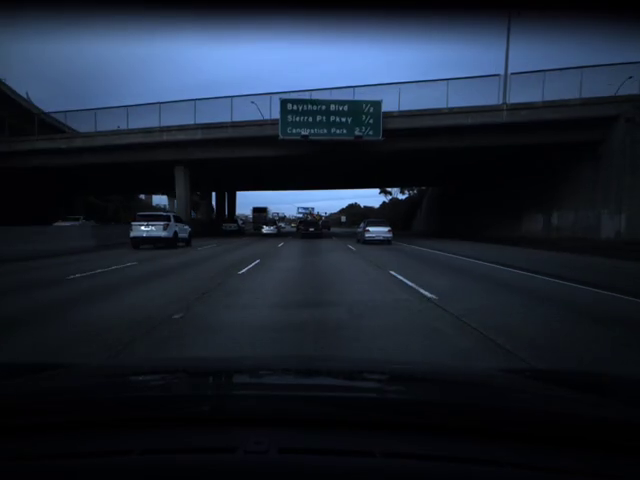
\includegraphics[width=.35\columnwidth]{./imgs/frame2_original.png}} \hspace{0.1cm}
  \subfloat[Frame after down sampling]{\label{figur:2}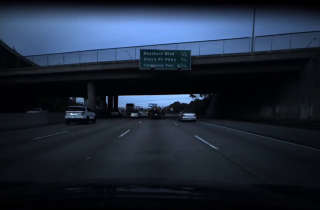
\includegraphics[width=.35\columnwidth]{./imgs/frame2_cut_sampled.png}}\\
  \subfloat[Optical flow field, already down sampled]{\label{figur:3}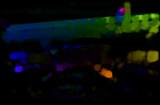
\includegraphics[width=0.7\columnwidth]{./imgs/frame2_flow_field.png}}
  \label{figur}\caption{Preprocessing of the video frames.}
\end{figure}

Explain, how we display the optical flow.

\section{Method selection and architecture}
Used MSE as performance metric

The prediction of the vehicles speed is a non-linear regression task, the choice of a neural network is reasonable. Recent 
architectures we discussed in the lecture (RESNET, GOOGLENET, etc.) have shown than using multiple stacked convolution layers
combined with stacked dense layers, perform well on image classification tasks. Therefore the choice of a convolutional neural network
is justified.

As a base architecture we decided to give the model of https://arxiv.org/pdf/1604.07316v1.pdf a try. As the paper used it
for self-driving cars, the model has enough complexity to handle a task like ours and with the amount of layers, we had a lot of
possibilities, to fine-tune and improve the model.

In a first approach, we tried the raw model, using different activation functions and we embedded residual layer and batch 
normalization as improvements we discussed in the lecture, to speed up training and improve the performance. As proposed in the lecture
we used
\begin{align*}
\mathrm{ReLu}: \mathbb{R} \to \mathbb{R}_0^+, x \mapsto \max\{0,x\}
\end{align*}
as the initial activation function. We used batch normalization according to https://arxiv.org/pdf/1502.03167.pdf, to speed up the 
training process. Using the ReLU function and XX epochs for training, we achieved a MSE of around 12, running the code multiple times, to ensure this result holds. This result was not really promising, so we wanted to improve the error firstly modifying the model.

To solve the problem of dead neurons\footnote{As one can clearly see in the defintion of the ReLU 
function, neurons with a value below zero cannot participate in the learning process.} of the ReLU function, we 
tried the leakyReLU function
\begin{align*}
\mathrm{leakyReLU} : \mathbb{R} \to \mathbb{R}, x \mapsto \begin{cases}
x, x \geq 0\\
c \cdot x, x <0
\end{cases}
\end{align*}
with a parameter $c = 0.01$. Using again batch normalization, we achieved an error of around 10.

ASSUMPTION TRAINING ERROR UNDER 3 IS EXTREMLY GOOD, to avoid overfit

MAYBE PROVIDE TABULAR WITH TRAIN AND TEST ERROR

MISSING ANALYSIS OF THE DATA SET

relatively low number of epochs, as the model always seemed to overfit, because we have a relatively complex model for not a lot of
data frames



\section{Results and comparison}

\section{Further work}

%\begin{table}[htbp]
%\caption{Table Type Styles}
%\begin{center}
%\begin{tabular}{|c|c|c|c|}
%\hline
%\textbf{Table}&\multicolumn{3}{|c|}{\textbf{Table Column Head}} \\
%\cline{2-4} 
%\textbf{Head} & \textbf{\textit{Table column subhead}}& \textbf{\textit{Subhead}}& \textbf{\textit{Subhead}} \\
%\hline
%copy& More table copy$^{\mathrm{a}}$& &  \\
%\hline
%\multicolumn{4}{l}{$^{\mathrm{a}}$Sample of a Table footnote.}
%\end{tabular}
%\label{tab1}
%\end{center}
%\end{table}



%Figure Labels: Use 8 point Times New Roman for Figure labels. Use words 
%rather than symbols or abbreviations when writing Figure axis labels to 
%avoid confusing the reader. As an example, write the quantity 
%``Magnetization'', or ``Magnetization, M'', not just ``M''. If including 
%units in the label, present them within parentheses. Do not label axes only 
%with units. In the example, write ``Magnetization (A/m)'' or ``Magnetization 
%\{A[m(1)]\}'', not just ``A/m''. Do not label axes with a ratio of 
%quantities and units. For example, write ``Temperature (K)'', not 
%``Temperature/K''.

\section*{Acknowledgment}





\begin{thebibliography}{00}
\bibitem{b1} G. Eason, B. Noble, and I. N. Sneddon, ``On certain integrals of Lipschitz-Hankel type involving products of Bessel functions,'' Phil. Trans. Roy. Soc. London, vol. A247, pp. 529--551, April 1955.
\bibitem{b2} J. Clerk Maxwell, A Treatise on Electricity and Magnetism, 3rd ed., vol. 2. Oxford: Clarendon, 1892, pp.68--73.
\bibitem{b3} I. S. Jacobs and C. P. Bean, ``Fine particles, thin films and exchange anisotropy,'' in Magnetism, vol. III, G. T. Rado and H. Suhl, Eds. New York: Academic, 1963, pp. 271--350.
\bibitem{b4} K. Elissa, ``Title of paper if known,'' unpublished.
\bibitem{b5} R. Nicole, ``Title of paper with only first word capitalized,'' J. Name Stand. Abbrev., in press.
\bibitem{b6} Y. Yorozu, M. Hirano, K. Oka, and Y. Tagawa, ``Electron spectroscopy studies on magneto-optical media and plastic substrate interface,'' IEEE Transl. J. Magn. Japan, vol. 2, pp. 740--741, August 1987 [Digests 9th Annual Conf. Magnetics Japan, p. 301, 1982].
\bibitem{b7} M. Young, The Technical Writer's Handbook. Mill Valley, CA: University Science, 1989.
\end{thebibliography}


\end{document}
